\documentclass{article}
\usepackage[utf8]{inputenc}
\usepackage{multicol}
\usepackage[formats]{listings}
\lstloadaspects{formats}
\usepackage{verbatim}
\usepackage{color}
\usepackage{geometry}
\usepackage{float}
\usepackage{amsmath}
\usepackage{multirow}% http://ctan.org/pkg/multirow
\usepackage{hhline}% http://ctan.org/pkg/hhline
\usepackage{caption}
\usepackage{pdflscape}
\usepackage{caption}
\usepackage[font={color=black},figurename=Fig.,labelfont={it}]{caption}
\usepackage{hyperref}
\setlength{\belowcaptionskip}{-10pt}
\setlength{\abovecaptionskip}{-30pt}
\floatstyle{boxed} 
\restylefloat{figure}
\usepackage{graphicx}
\usepackage{subcaption}
\definecolor{codegreen}{rgb}{0,0.6,0}
\definecolor{codegray}{rgb}{0.5,0.5,0.5}
\definecolor{codepurple}{rgb}{0.58,0,0.82}
\definecolor{backcolour}{rgb}{0.95,0.95,0.92}
\lstdefinestyle{mystyle}{
	backgroundcolor=\color{backcolour},   
	commentstyle=\color{codegreen},
	keywordstyle=\color{blue},
	numberstyle=\tiny\color{codegray},
	stringstyle=\color{codepurple},
	basicstyle=\footnotesize,
	breakatwhitespace=false,         
	breaklines=true,                 
	captionpos=b,                    
	keepspaces=true,                 
	numbers=left,                    
	numbersep=5pt,                  
	showspaces=false,                
	showstringspaces=false,
	showtabs=false,                  
	tabsize=2
}
\lstset{style=mystyle}
\title{Image Processing\\
	Home work 08}
\author{Aqeel Labash\\ \textbf{Lecturer:} Gholamreza Anbarjafari}
\geometry{
	a4paper,
	total={170mm,257mm},	
	left=10mm,
	top=5mm,
}
\begin{document}
	\maketitle
\begin{figure}[H]
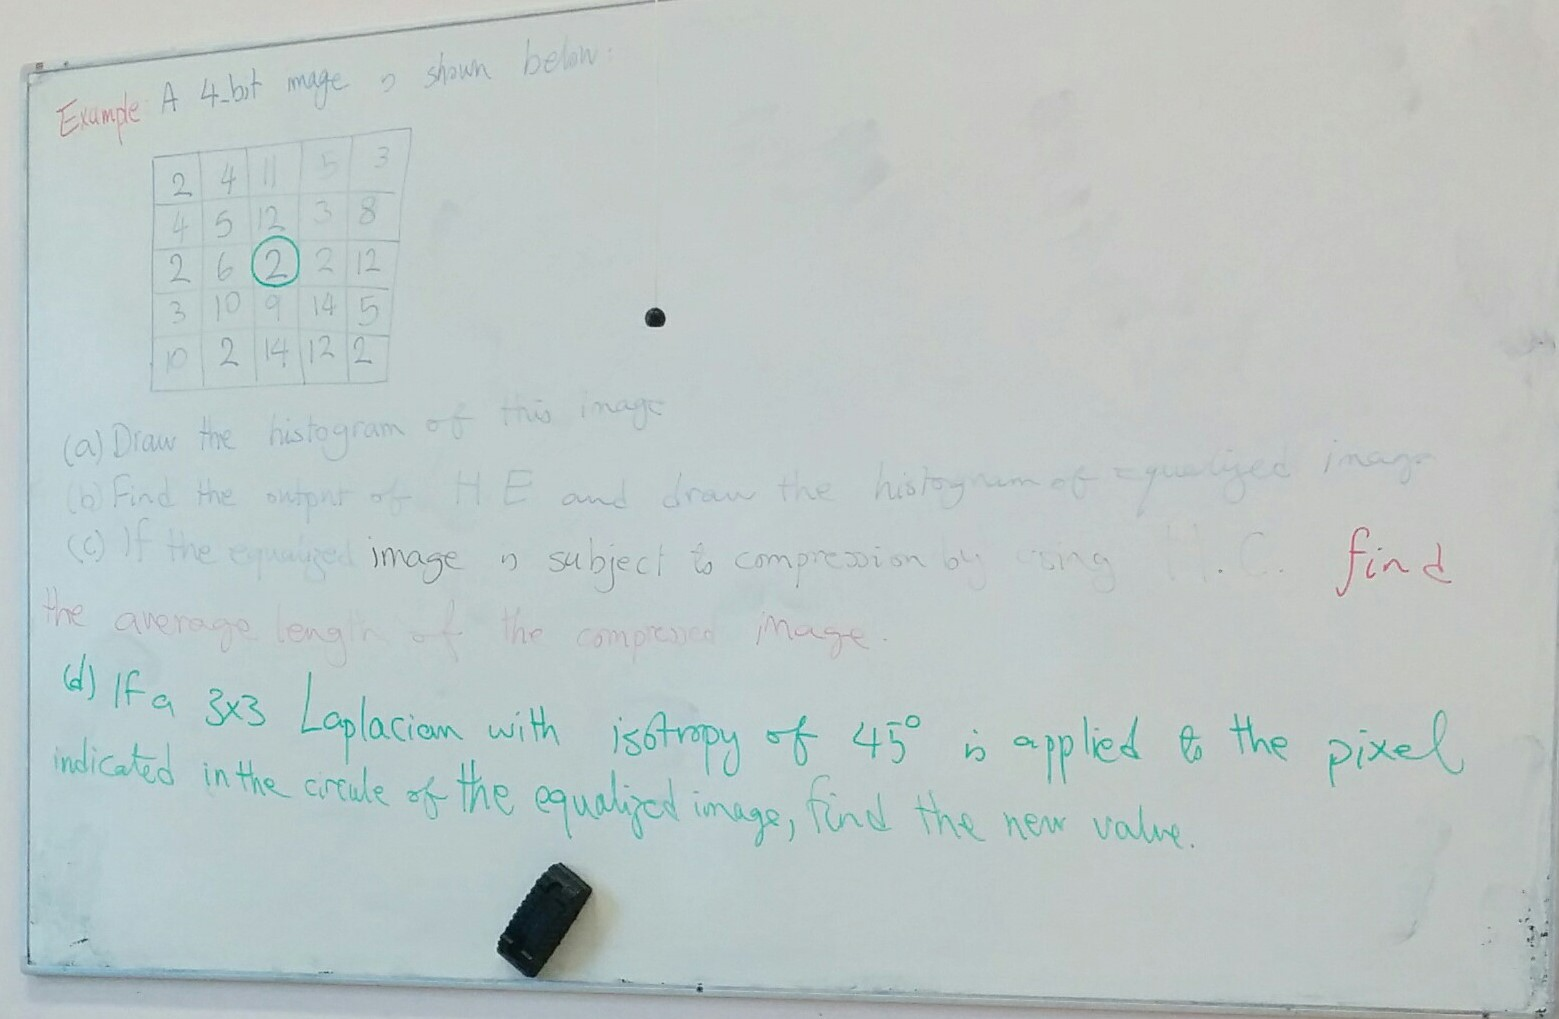
\includegraphics[scale=0.415]{Questions.jpg}
\end{figure}
\section*{A}
The histogram is just the frequency vs Value. The values as in the following table : \\
\begin{tabular}{|c|c|}
\hline
Value &Count\\ \hline
2&6\\ \hline 
3&3\\ \hline 
4&2\\ \hline 
5&3\\ \hline 
6&1\\ \hline 
8&1\\ \hline 
9&1\\ \hline 
10&2\\ \hline 
11&1\\ \hline  
12&3\\ \hline 
14&2 \\ \hline
\end{tabular}
 
 \begin{figure}[H]
 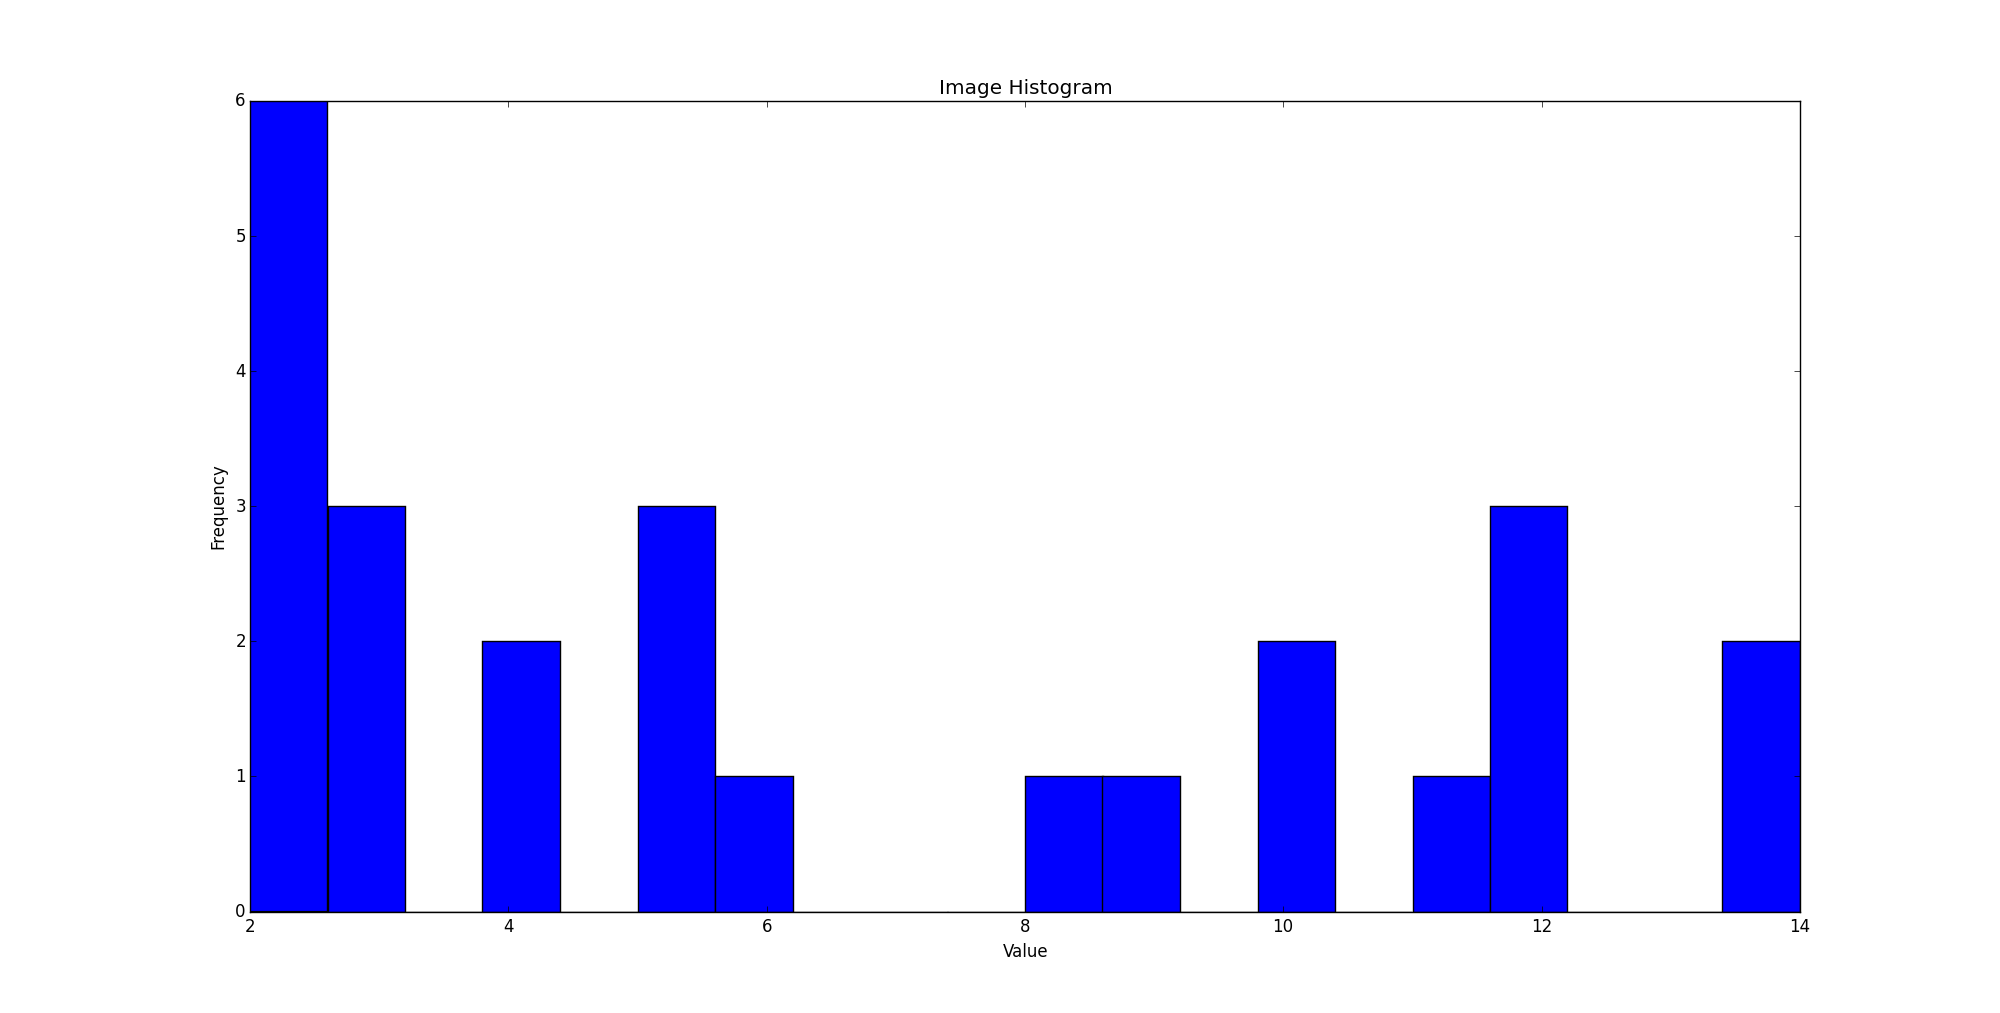
\includegraphics[trim={5cm 0cm 5cm 0cm},clip,scale=0.35]{histogram_py.png}
 \caption{Histogram of the image}
 \end{figure}
 \section *{B}
First here is the values :\\
\begin{tabular}{|c|c|c|c|c|}
\hline
value&Count&Probablitiy&CDF&HE\\ \hline 
 2&6&0.24&0.24&0\\ \hline 
 3&3&0.12&0.36&2\\ \hline 
 4&2&0.08&0.44&4\\ \hline 
 5&3&0.12&0.56&6\\ \hline 
 6&1&0.04&0.60&7\\ \hline 
 8&1&0.04&0.64&8\\ \hline 
 9&1&0.04&0.68&9\\ \hline 
 10&2&0.08&0.76&10\\ \hline 
 11&1&0.04&0.80&11\\ \hline 
 12&3&0.12&0.92&13\\ \hline 
 14&2&0.08&1.00&15 \\ \hline
\end{tabular}\\
And here is the historam of the equalized image : 
 \begin{figure}[H]
 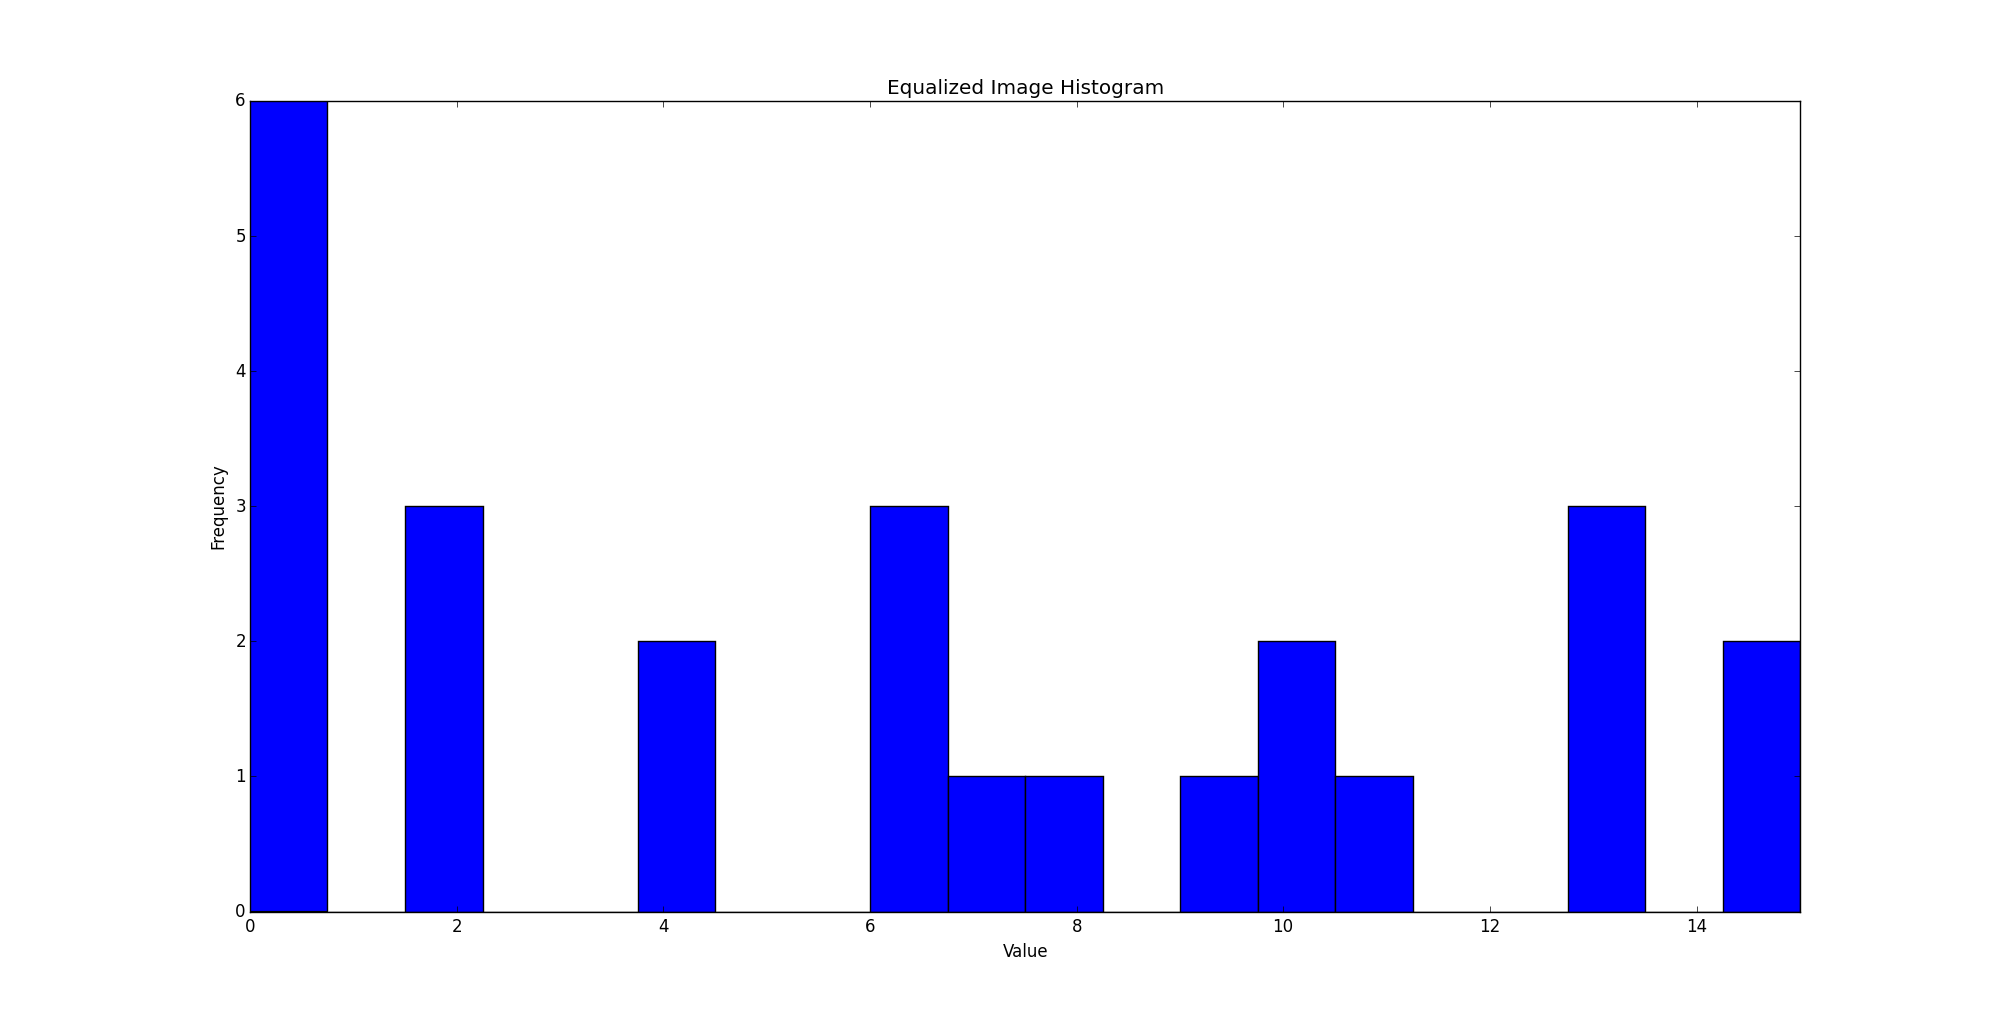
\includegraphics[trim={5cm 0cm 5cm 0cm},clip,scale=0.4]{histogram_eq.png}
 \caption{Histogram of the equalized image}
 \end{figure}
 \section *{C}
For Huffman coding I found a way with numbers (same as probabilities but just with counts). I made the draw on the board here is the image :
\begin{figure}[H]
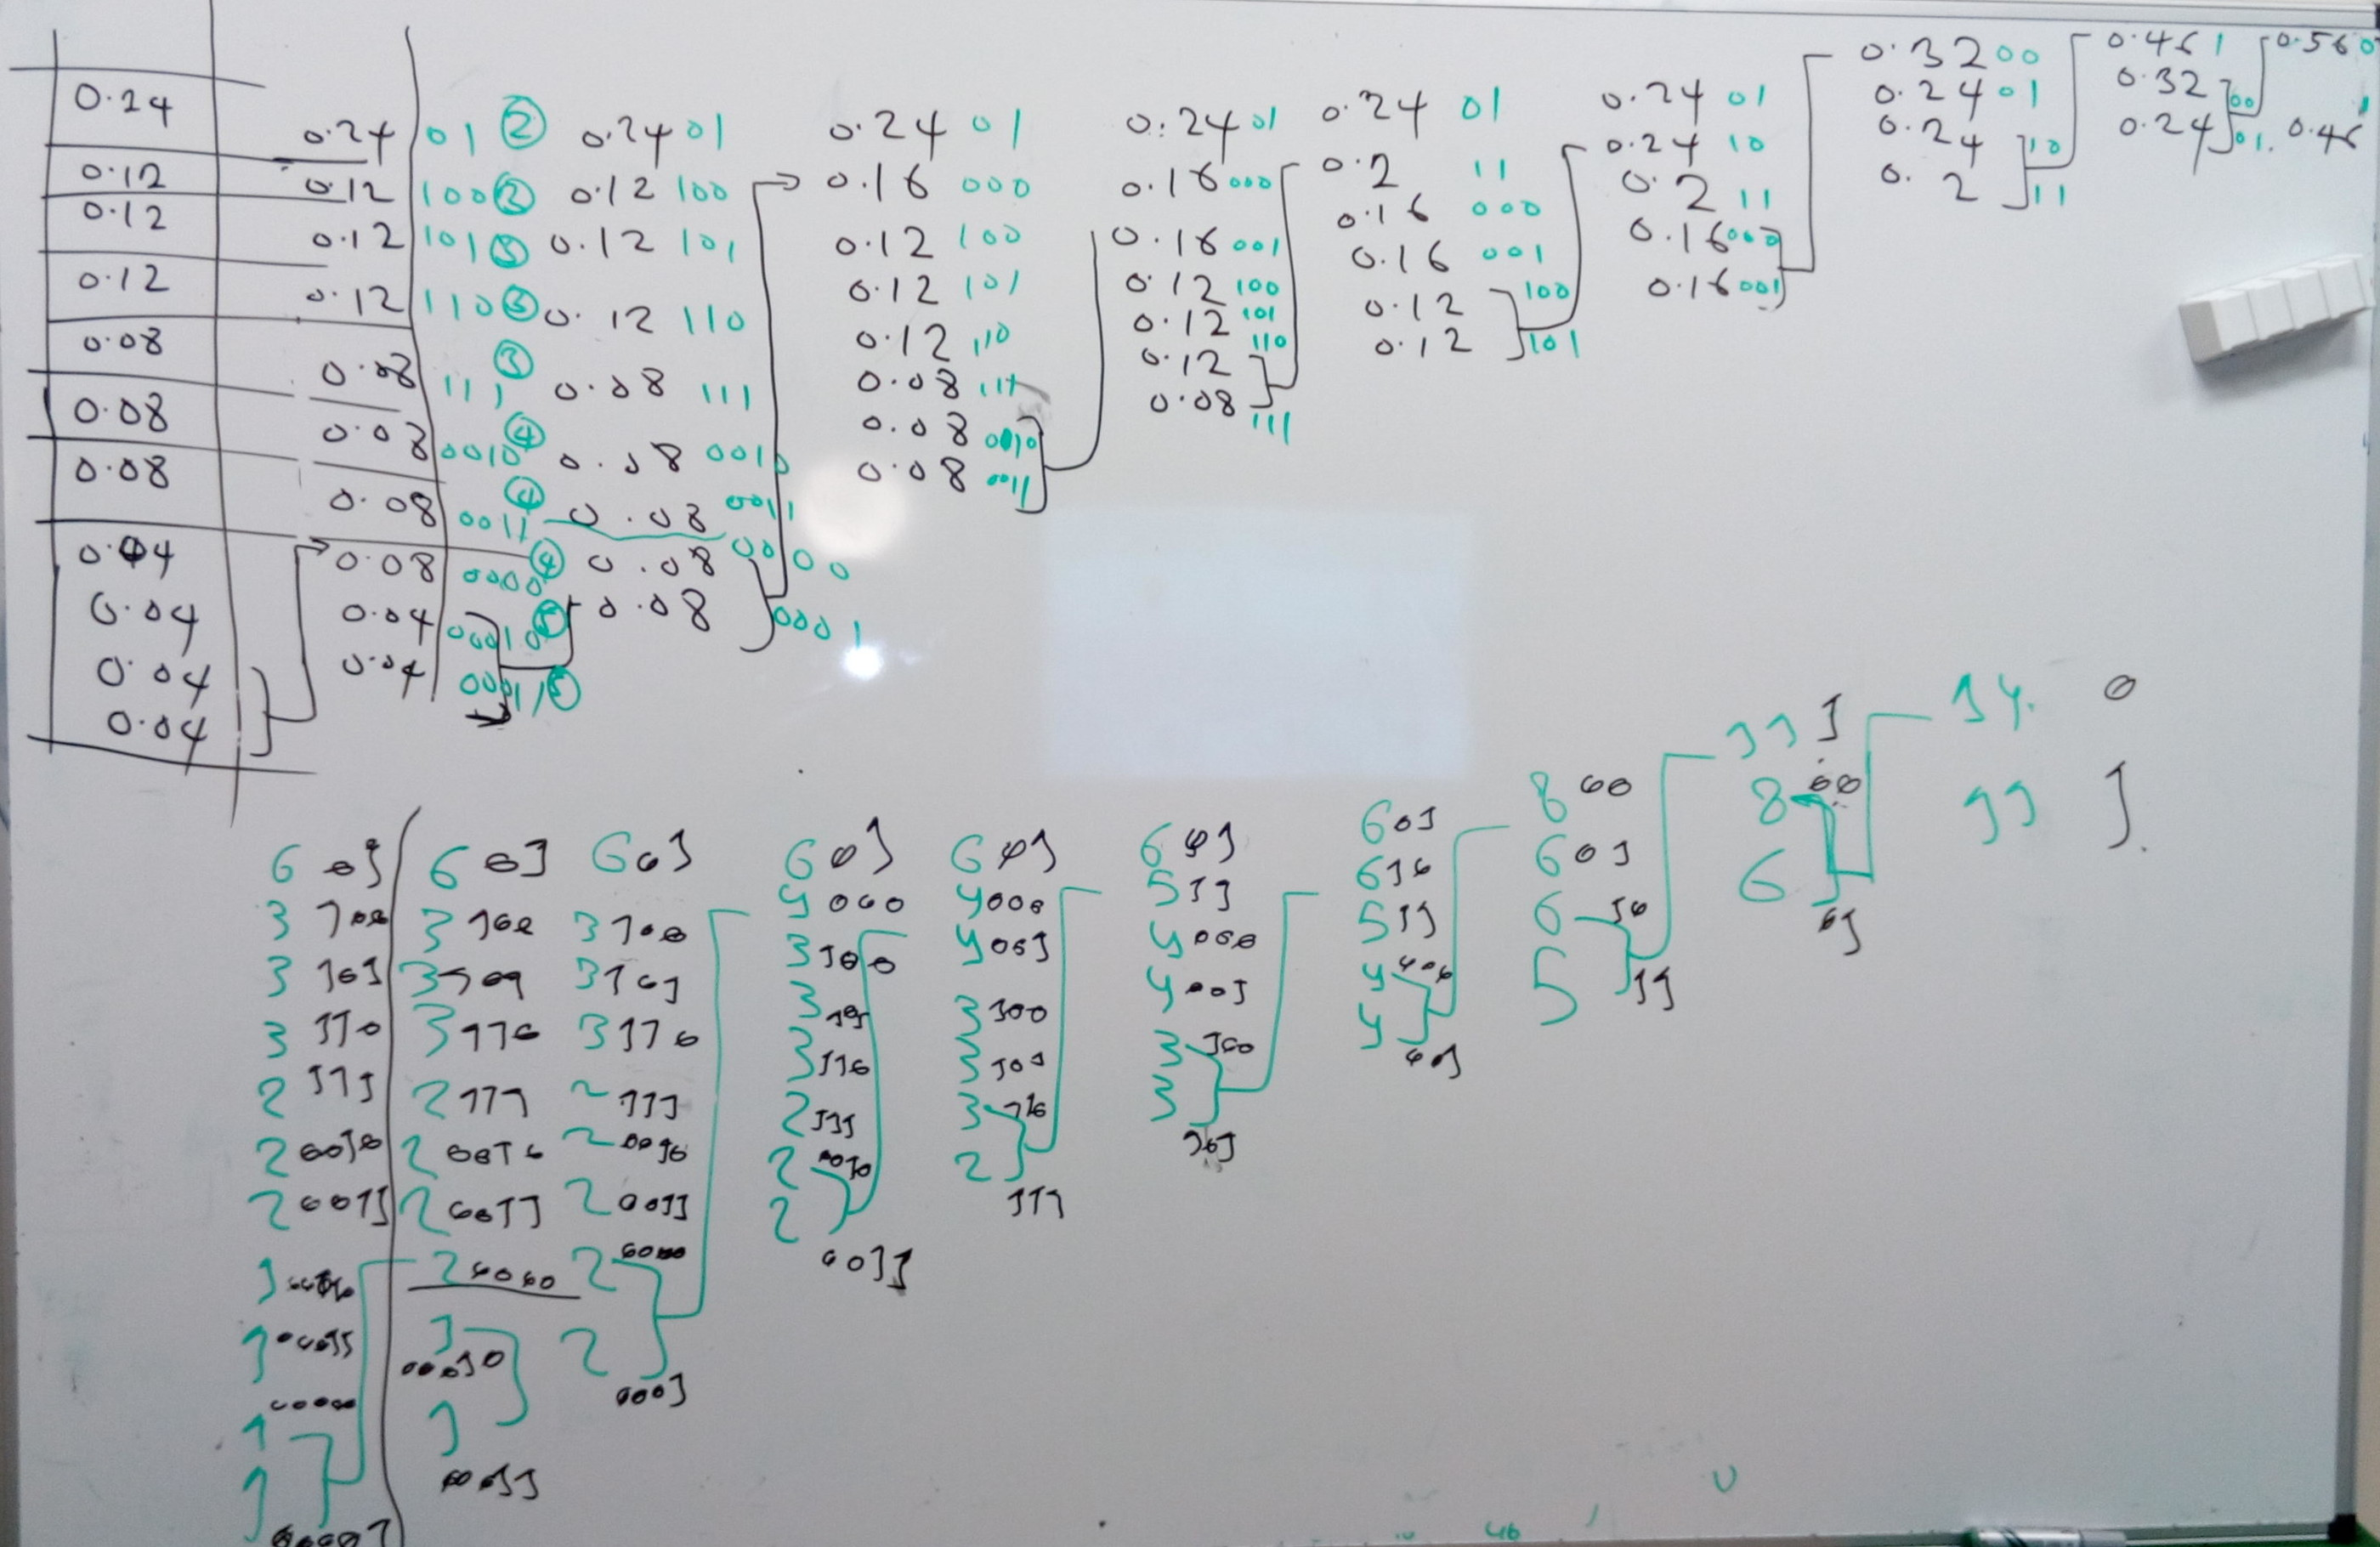
\includegraphics[scale=0.2]{c_modified.jpg}
\caption{The process of building Huffman Code}
\end{figure}
Here is the values:\\ \\ 
\begin{tabular}{|c|c|c|c|}
\hline
value&Count&Pr&Code\_Length\\ \hline 
0&6&0.24&2\\ \hline 
2&3&0.12&3\\ \hline 
6&3&0.12&3\\ \hline 
13&3&0.12&5\\ \hline 
4&2&0.08&3\\ \hline 
10&2&0.08&5\\ \hline 
15&2&0.08&5\\ \hline 
7&1&0.04&3\\ \hline 
8&1&0.04&4\\ \hline 
9&1&0.04&4\\ \hline 
11&1&0.04&5\\ \hline
\end{tabular} \\

From the previous table we can see that Average length is 3.4800000000000004~ 3.48\\
\textbf{Note:} For more details please check my solution file (HTML in python with figures + tables at )
\end{document}